\documentclass[a4paper,10pt]{article}
\usepackage[margin=17mm,headheight=13pt,headsep=5mm,footskip=9mm]{geometry}
\usepackage[T1]{fontenc}
\usepackage{lmodern,amsmath,amssymb,graphicx,tikz,microtype,fancyhdr}
\usetikzlibrary{arrows.meta,calc}
\usepackage[colorlinks=true,linkcolor=black]{hyperref}
\hypersetup{pdftitle={CuRo6R -- Analytical IK illustrations},pdfsubject={Geometric derivation: frame change, invariants and shoulder-angle recovery}}
\definecolor{dhink}{HTML}{243747}
\definecolor{dhblue}{HTML}{2164A1}
\definecolor{dhred}{HTML}{B84338}
\definecolor{dhgreen}{HTML}{337A55}
\definecolor{dhgold}{HTML}{A66816}
\definecolor{dhpurple}{HTML}{79509A}
\definecolor{dhgray}{HTML}{78838C}
\pagestyle{fancy}
\fancyhf{}
\fancyhead[L]{\small\sffamily CuRo6R\enspace |\enspace Analytical inverse kinematics}
\fancyhead[R]{\small\sffamily Illustration preview}
\fancyfoot[C]{\small\thepage}
\renewcommand{\headrulewidth}{.3pt}
\setlength{\parindent}{0pt}
\setlength{\parskip}{5pt}
\newcommand{\IKPanel}[1]{\resizebox{\linewidth}{!}{\input{figures/#1}}}
\begin{document}
{\Large\bfseries From the physical arm to the position equations}

The same configuration is used throughout:
$q_1=40^\circ$, $q_2=25^\circ$, $q_3=75^\circ$ and $\gamma=30^\circ$.
Each panel isolates one geometric idea used in the derivation.

\begin{minipage}[t]{.485\linewidth}
 {\bfseries (a) Locating the shoulder frame}\par
 \IKPanel{ik_base_frame}
 {\small The shoulder frame has origin $S$. Its orientation includes $q_1$
 and the fixed roll $\gamma$, which tilts $\bar y=R_z(q_1)e_y$ into $y_s$.
 It is independent of $q_2$.}
\end{minipage}\hfill
\begin{minipage}[t]{.485\linewidth}
 {\bfseries (b) Why $q_2$ can be eliminated}\par
 \IKPanel{ik_shoulder_frame}
 {\small In the shoulder frame, $u$ is the wrist vector at $q_2=0$ and
 $r=R_y(q_2)u$. The rotation preserves the axial coordinate $Y$ and the squared
 distance $N=\|r\|^2$.}
\end{minipage}

\vspace{2mm}
\begin{center}
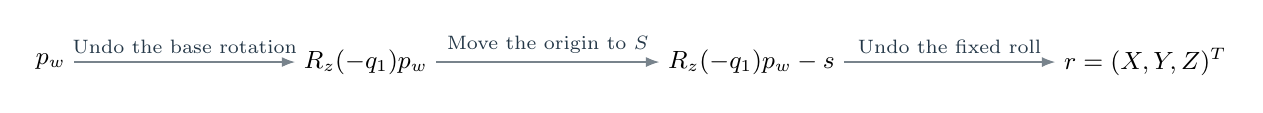
\begin{tikzpicture}[font=\small,>=Latex,every node/.style={inner sep=3pt}]
 \node (a) at (0,0) {$p_w$};
 \node (b) at (4.0,0) {$R_z(-q_1)p_w$};
 \node (c) at (8.9,0) {$R_z(-q_1)p_w-s$};
 \node (d) at (13.9,0) {$r=(X,Y,Z)^T$};
 \draw[->,dhgray] (a) -- node[above,font=\scriptsize,text=dhink]{Undo the base rotation} (b);
 \draw[->,dhgray] (b) -- node[above,font=\scriptsize,text=dhink]{Move the origin to $S$} (c);
 \draw[->,dhgray] (c) -- node[above,font=\scriptsize,text=dhink]{Undo the fixed roll} (d);
\end{tikzpicture}
\end{center}
\vspace{-1mm}
\[
 s=(a_1,0,d_1)^T,\qquad
 r=R_x(-\gamma)\bigl(R_z(-q_1)p_w-s\bigr).
\]

\begin{minipage}[t]{.485\linewidth}
 {\bfseries (c) Recovering $q_2$ in the $x_sz_s$ plane}\par
 \IKPanel{ik_shoulder_projection}
\end{minipage}\hfill
\begin{minipage}[t]{.475\linewidth}
 \vspace{4mm}
 With $A=a_2+d_4c_3$, the reference vector is $u=(A,Y,d_3)^T$.
 Panel (c) drops the common $y_s$ component. The planar rotation gives
 \[
 \begin{aligned}
 X&=A\cos q_2+d_3\sin q_2,\\
 Z&=-A\sin q_2+d_3\cos q_2.
 \end{aligned}
 \]
 Combining these equations isolates a scaled cosine and sine:
 \[
 \begin{aligned}
 AX+d_3Z&=(A^2+d_3^2)\cos q_2,\\
 d_3X-AZ&=(A^2+d_3^2)\sin q_2.
 \end{aligned}
 \]
 Their common factor $A^2+d_3^2$ is positive, so applying
 $\operatorname{atan2}$ to these scaled sine and cosine values gives
 \[
 q_2=\operatorname{atan2}(d_3X-AZ,\,AX+d_3Z).
 \]
\end{minipage}

\vspace{3mm}
{\small\textbf{Geometry and notation.}
 Point locations and frame orientations follow the CuRo6R URDF. The faint arm
 outline provides context; panels (b) and (c) show the vectors needed for the
 derivation. Gold denotes the reference vector at $q_2=0$ and purple denotes
 the vector after the shoulder rotation.}
\end{document}
